\begin{DoxyVerb}Button example will display a button widget then poll for button presses and update screen <br>
\end{DoxyVerb}
  
\begin{DoxyImageNoCaption}
  \mbox{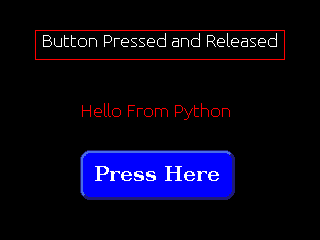
\includegraphics{button.png}}
\end{DoxyImageNoCaption}
 
\begin{DoxyCodeInclude}
1 \textcolor{comment}{# Button ezLCD Python demo}
2 \textcolor{comment}{#}
3 
4 \textcolor{keyword}{import} platform
5 \textcolor{keyword}{import} sys
6 sys.path.append(\textcolor{stringliteral}{'module'}) 
7 \textcolor{keyword}{from} ezLCD3xx \textcolor{keyword}{import} *
8 
9 LCD = ezLCD(\textcolor{keywordtype}{None}) 
10 comPort =  LCD.findezLCD()
11 
12 \textcolor{comment}{#check what OS we are on}
13 \textcolor{comment}{#Windows}
14 \textcolor{keywordflow}{if} platform.system() == \textcolor{stringliteral}{'Windows'}:
15     LCD = ezLCD(comPort[0][0])
16 \textcolor{comment}{#Mac}
17 \textcolor{keywordflow}{elif} platform.system() == \textcolor{stringliteral}{'Dawrwin'}:
18     LCD = ezLCD(\textcolor{stringliteral}{'/dev/tty.usbsomething'})
19 \textcolor{comment}{#Linux}
20 \textcolor{keywordflow}{elif} platform.system() == \textcolor{stringliteral}{'Linux'}:
21     LCD = ezLCD(\textcolor{stringliteral}{'/dev/ttyACM0'})
22 
23 \textcolor{comment}{# Bail out if comport error}
24 \textcolor{keywordflow}{if} LCD.openSerial()==\textcolor{keyword}{False}:
25     \textcolor{keywordflow}{print} \textcolor{stringliteral}{'Error Opening Port'}
26     \textcolor{keywordflow}{raise} SystemExit
27 
28 \textcolor{comment}{# Turn verbose off }
29 LCD.verbose(OFF)
30 \textcolor{comment}{# Turn off button press info from ezLCD}
31 LCD.wquiet(ON)
32 \textcolor{comment}{# CLear screen}
33 LCD.cls()
34 \textcolor{comment}{# Set draw color to red}
35 LCD.color(RED)
36 \textcolor{comment}{# Set widget font 0}
37 LCD.fontw(0,\textcolor{stringliteral}{'1'})
38 \textcolor{comment}{# Set wodget font 1}
39 LCD.fontw(1,\textcolor{stringliteral}{'0'})
40 \textcolor{comment}{# Set theme #1 }
41 LCD.theme(1, 155, 152, 3, 0, 3, 24, 4, 5, 0, 1)
42 \textcolor{comment}{# Print string at coordinates x=80 and y=100}
43 LCD.printString(\textcolor{stringliteral}{"Hello From Python"},80,100)
44 \textcolor{comment}{# Draw button widget with a ID of 1}
45 LCD.button( 1,  80, 150, 155, 50, 1, 0, 10, 6, 3,\textcolor{stringliteral}{'Press Here'})
46 \textcolor{comment}{# Draw a staticText box}
47 LCD.staticText(2, 35, 30, 250, 30, 8, 1, 1,\textcolor{stringliteral}{'Press Button'})
48 \textcolor{comment}{# Clear widget stack}
49 LCD.wstack(CLEAR)
50 \textcolor{keywordflow}{while} \textcolor{keyword}{True}:
51     \textcolor{comment}{# check widget stack this will return widget updates (button press ect.) last in first out order}
52     (ID, Info, Data) = LCD.wstack(FIFO)
53 \textcolor{comment}{#   print ID, Info, Data}
54     \textcolor{comment}{# check if ID = 1 widget 1 and info = pressed }
55     \textcolor{keywordflow}{if} ID == 1 \textcolor{keywordflow}{and} Info == 4:
56         \textcolor{comment}{# clear the stack just to be safe}
57 \textcolor{comment}{#       LCD.wstack(CLEAR)}
58         \textcolor{comment}{# change draw color to yellow}
59         LCD.color(YELLOW)
60         \textcolor{comment}{# change change string 1 for text on static text ID 2}
61         LCD.string(1,\textcolor{stringliteral}{'Button Pressed'})
62         \textcolor{comment}{# redraw static text box ID 2 3=redraw      }
63         LCD.wstate(2, 3)
64     \textcolor{comment}{# check if ID = 1 widget 1 and info = pressed and released}
65     \textcolor{keywordflow}{if} ID == 1 \textcolor{keywordflow}{and} Info == 1:
66         \textcolor{comment}{# clear the stack just to be safe}
67 \textcolor{comment}{#       LCD.wstack(CLEAR)}
68         \textcolor{comment}{# change draw color to yellow}
69         LCD.color(YELLOW)
70         \textcolor{comment}{# change change string 1 for text on static text ID 2}
71         LCD.string(1,\textcolor{stringliteral}{'Button Pressed and Released'})
72         \textcolor{comment}{# redraw static text box ID 2 3=redraw}
73         LCD.wstate(2, 3)
74 
75         
\end{DoxyCodeInclude}
 Load example will display the cpu load as a graph \par
  
\begin{DoxyImageNoCaption}
  \mbox{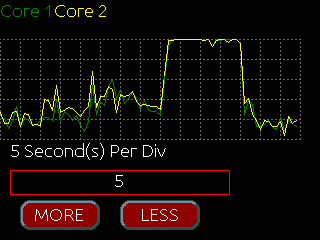
\includegraphics{load.png}}
\end{DoxyImageNoCaption}
 
\begin{DoxyCodeInclude}
1 \textcolor{comment}{#!/usr/bin/env python}
2 \textcolor{comment}{# Python Serial library for ezLCD3xx}
3 \textcolor{comment}{# http://www.ezlcd.com/}
4 \textcolor{comment}{#}
5 \textcolor{comment}{# You need the pySerial Library by Chris Liechti}
6 \textcolor{comment}{# http://pyserial.wiki.sourceforge.net/pySerial}
7 \textcolor{comment}{#}
8 
9 
10 \textcolor{comment}{# END SerLCD Class Definition --------------------------------------}
11 
12 \textcolor{comment}{# Start Test Program -----------------------------------------------}
13 \textcolor{keyword}{import} commands
14 \textcolor{keyword}{import} os
15 \textcolor{keyword}{import} re
16 \textcolor{keyword}{import} time \textcolor{keyword}{as} timer
17 \textcolor{keyword}{import} sys
18 \textcolor{keyword}{import} platform
19 \textcolor{keyword}{import} time
20 \textcolor{keyword}{import} psutil
21     
22 sys.path.append(\textcolor{stringliteral}{'module'}) 
23 \textcolor{keyword}{from} ezLCD3xx \textcolor{keyword}{import} *
24 
25 \textcolor{keyword}{def }drawGrid():
26     LCD.lineType(2)
27     LCD.xy(0,30)
28     LCD.color(BLACK)
29     LCD.box(300,110,1)
30     LCD.xy(0,0)
31     LCD.color(GREEN)
32     LCD.printString(\textcolor{stringliteral}{'Core 1'})
33     LCD.color(YELLOW)
34     LCD.printString(\textcolor{stringliteral}{'  Core 2'})
35     LCD.color(155)
36     LCD.color(LIME)
37     LCD.font(\textcolor{stringliteral}{'1'})
38     LCD.font(\textcolor{stringliteral}{'0'})
39     LCD.color(151)
40     \textcolor{keywordflow}{for} y \textcolor{keywordflow}{in} range(6):
41         LCD.xy(0,(y*20)+39)
42         LCD.line(300,(y*20)+39)
43     \textcolor{keywordflow}{for} x \textcolor{keywordflow}{in} range(16):
44         LCD.xy(x*20,39)
45         LCD.line(x*20,139)
46     LCD.xy(300,39)
47     LCD.line(300,139)
48     LCD.lineType(0)
49     
50 \textcolor{keyword}{def }drawTime(res):
51     LCD.xy(10,140)
52     LCD.color(BLACK)
53     LCD.box(300,30, FILLED)
54     LCD.color(WHITE)
55     Time=str(res)+\textcolor{stringliteral}{' Second(s) Per Div'}
56     LCD.printString(Time)
57 
58     LCD.string(5, str(res))
59     LCD.wstate(7,REDRAW)
60 
61 LCD = ezLCD(\textcolor{keywordtype}{None}) 
62 comPort =  LCD.findezLCD()
63 
64 \textcolor{comment}{#check what OS we are on}
65 \textcolor{comment}{#Windows}
66 \textcolor{keywordflow}{if} platform.system() == \textcolor{stringliteral}{'Windows'}:
67     LCD = ezLCD(comPort[0][0])
68 \textcolor{comment}{#Mac}
69 \textcolor{keywordflow}{elif} platform.system() == \textcolor{stringliteral}{'Dawrwin'}:
70     LCD = ezLCD(\textcolor{stringliteral}{'/dev/tty.usbsomething'})
71 \textcolor{comment}{#Linux}
72 \textcolor{keywordflow}{elif} platform.system() == \textcolor{stringliteral}{'Linux'}:
73     LCD = ezLCD(\textcolor{stringliteral}{'/dev/ttyACM0'})
74 \textcolor{comment}{# Bail out if comport error}
75 \textcolor{keywordflow}{if} LCD.openSerial()==\textcolor{keyword}{False}:
76     \textcolor{keywordflow}{print} \textcolor{stringliteral}{'Error Opening Port'}
77     \textcolor{keywordflow}{raise} SystemExit
78 
79 LCD.ping()
80 LCD.verbose(\textcolor{stringliteral}{'OFF'})
81 LCD.wquiet(ON)
82 LCD.cls()
83 LCD.fontw(0,\textcolor{stringliteral}{'1'})
84 LCD.fontw(1,\textcolor{stringliteral}{'0'})
85 LCD.fontw(2,\textcolor{stringliteral}{'serif24'})
86 LCD.theme(1, 155, 152, 3, 0, 3, 24, 4, 5, 0, 1)
87 LCD.backlight(100, 5, 10)
88 LCD.cls()
89 LCD.font(\textcolor{stringliteral}{'0'})
90 LCD.fonto(0)
91 info = \textcolor{stringliteral}{' '}
92 LCD.string( 1, \textcolor{stringliteral}{'%'})
93 LCD.color(WHITE)
94 LCD.cfgio(8,\textcolor{stringliteral}{'analog'})
95 \textcolor{keywordflow}{print} LCD.xmax()
96 \textcolor{keywordflow}{print} LCD.ymax()
97 \textcolor{keywordflow}{print} LCD.string(65)
98 \textcolor{keywordflow}{print} LCD.string(66)
99 
100 
101 LCD.button( 5, 20, 200, 80, 30 , 1, 0, 10, 1, 2, \textcolor{stringliteral}{'MORE'})
102 LCD.button( 6, 120, 200, 80, 30 , 1, 0, 10, 1, 3, \textcolor{stringliteral}{'LESS'})
103 LCD.staticText(7, 10, 170, 220, 25, 8, 1, 5, \textcolor{stringliteral}{'test'})
104 drawGrid()
105 x=0
106 y1=239
107 y2=239
108 lx=0
109 ly1=239
110 ly2=239
111 res=5
112 drawTime(res)   
113 LCD.wstack(CLEAR)     
114 \textcolor{keywordflow}{while} \textcolor{keyword}{True}:
115 
116     oldinfo = info
117     cores=psutil.cpu\_percent(interval=1, percpu=\textcolor{keyword}{True})
118     y1 = 139 - cores[0]
119     y2 = 139 - cores[1]
120     \textcolor{keywordflow}{if} x!=0:
121         LCD.color(GREEN)
122         LCD.xy(lx,ly1)
123         LCD.line(x, y1)
124         LCD.color(YELLOW)
125         LCD.xy(lx,ly2)
126         LCD.line(x, y2)
127     ly1 = y1
128     ly2 = y2
129     lx = x   
130     x += 20/res
131     
132     \textcolor{keywordflow}{if} x >= 300:
133         x=0
134         y1=239
135         y2=239
136         lx =0
137         ly1 =239
138         ly2 =239
139         drawGrid()
140     (ID, info, data) = LCD.wstack(LIFO)
141     LCD.wstack(CLEAR)
142     \textcolor{keywordflow}{if} ID == 5 \textcolor{keywordflow}{and} info==1:
143         res +=1
144         drawTime(res)  
145     \textcolor{keywordflow}{if} ID == 6 \textcolor{keywordflow}{and} info==1:
146         \textcolor{keywordflow}{if} res > 1:
147             res -=1
148             drawTime(res)
149 LCD.closeSerial()
150 \textcolor{comment}{# End Test Program --------------------------------------}
\end{DoxyCodeInclude}
 